\section{Design}
\label{sec:intra-server}

Inspired by Unikernels~\cite{madhavapeddy2013unikernels}, we move networking and IPC functions from the kernel to user space. Similar to existing works~\cite{peter2016arrakis,jeong2014mtcp,libvma}, we leverage multiple queues in modern NICs to enable user-space direct access to network. %The kernel is still responsible for process creation, scheduling, virtual memory and device management, but no longer on the critical path of performance.
To maintain compatibility with existing Linux applications, we design a user-mode library \libipc as a drop-in replacement of the system call wrappers in the GNU C library (glibc). \libipc{} implements network socket functions in user mode, and adds a wrapper to other system calls to track process creation and memory allocation. \libipc{} is not considered a secure domain, as it shares memory space with the application. Figure~\ref{fig:architecture} shows the architecture of \sys{}.

Even though multiple threads in the same process share memory space, we still treat each thread as a separated process and use thread-specific storage to save states in \libipc. In the following text, unless explicitly mentioned, we use a ``process'' to refer to a regular process or a thread.

\subsection{Connection Management}
\label{subsec:socket-api}


%\subsubsection{Connection Creation}
%\label{subsubsec:connection_management}

\begin{figure}[t]
	\centering
	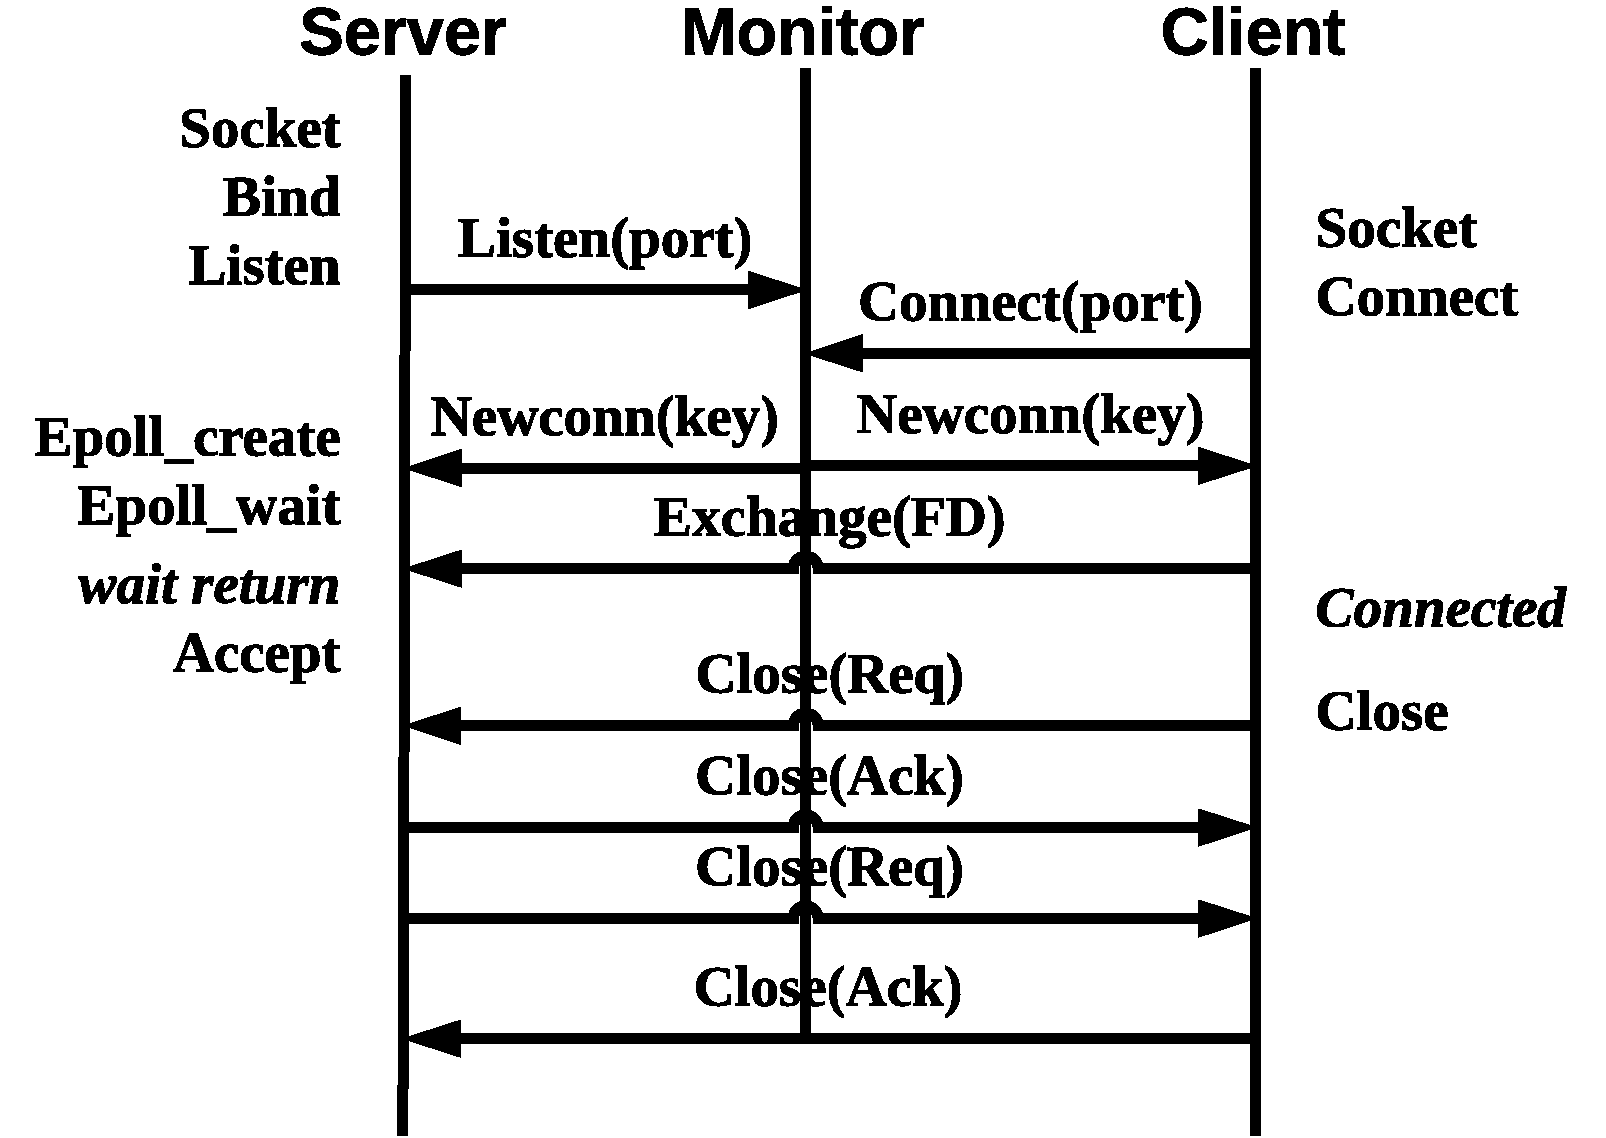
\includegraphics[width=0.45\textwidth]{images/conn-setup}
	\caption{The message flow of connection creation and close.}
	\label{fig:conn-setup}
	\vspace{-15pt}
\end{figure}

\parab{\texttt{Socket}.}
To create a socket connection, an application first calls \texttt{socket} to get a \textit{file descriptor} (FD). 
%Although Linux globally allocates the lowest available file descriptor, this property is rarely used~\cite{han2012megapipe,huang2017high}. We relax the semantics and maintains an FD table in each process. 
We maintains an FD table for each process. Upon allocation, \libipc{} finds an idle FD from the table or doubles the table size if none available. 
%The table is a vector of socket information with an allocation pointer, indexed by FD. Upon allocation, \libipc{} linearly moves the allocation pointer and finds the first idle FD. When the vector is more than half full, its size is doubled. This allows amortized O(1) allocation and O(1) lookup and deletion.
For multi-thread applications, since the FD namespace is shared, we partition the FD namespace to multiple ranges and each thread allocates FD in its range.
%Because per-FD information is local to a process, APIs on socket options are also local.

\parab{\texttt{Bind} and \texttt{listen}.}
A \emph{server} \texttt{bind}s a socket and needs to detect IP and port conflict. In this case, \texttt{bind} is non-partitionable. But a \emph{client} typically \texttt{bind}s without specifying IP and port, so we need to allocate a unique IP and port for it. For scalability, we partition the loopback IP address space (127.0.0.0/8) and each process allocates IP and port in its range.

\parab{\texttt{Connect} and \texttt{accept}.}
When a client connects to a server for the first time, it creates a Linux native \textit{bootstrap socket} to the monitor on destination server. Monitor identifies the client by peer IP and port. If the client is on the same server, they establish a shared memory queue. Otherwise, they establish an RDMA connection. Later communications between client and monitor go through shared memory or RDMA.

The monitor process distributes connection requests to listeners in a round-robin order, and the backlog is maintained in each listener. If monitor finds that it is the first time for client and listener to communicate, it creates a shared-memory queue for the process pair and sends the credentials to both processes. When a listener \texttt{accept}s a connection, it sends a message to sender via peer-to-peer shared-memory queue and the socket is established. As shown in Figure~\ref{fig:conn-setup}, connection creation takes three inter-process delays.

Distributing connection to listeners may lead to starvation when a listener does not \texttt{accept}. We devise a \textit{work stealing} approach. When a listener \texttt{accept}s from empty backlog, it requests the monitor to steal from others' backlog. To avoid polling empty backlogs, each listener notifies the monitor when its backlog becomes empty. To avoid contention between a listener and monitor, the monitor sends a request to the listener rather than stealing from the backlog directly.

%\subsubsection{Connection Close}

\parab{\texttt{Close} and \texttt{shutdown}.}
Connection close is a peer-to-peer operation because only the peer process needs to be notified. If FD is deleted immediately after \texttt{close}, a new connection may reuse the FD while the peer process might not yet have received the close event thus sends data to the wrong connection. To ensure the peer does not use the connection after a FD is deleted, we require a handshake between peers.
%Because socket is bidirectional, \texttt{close} is equivalent to \texttt{shutdown} on both send and receive directions. 
When the application shuts down a direction, it sends a \textit{shutdown message} to the peer. The peer shuts down the corresponding direction and responds with a shutdown message. A process deletes an FD when it has received shutdown messages in both directions.

%In order to achieve high scalability, we separate scalable operations to different processes. To avoid the overhead of contention, \libipc enable the file descriptor allocation by individual process and when a connection is setup, the other peer of the connection gets notified of the file descriptor number by message passing. Since we treat different threads in one process as different processes, we allocate file descriptor of different ranges to each of them to avoid collision. Since file descriptor is managed separately by each process, it is possible that a file descriptor is reused after the connection is closed. Our solution is that resources of a file descriptor is not released until an ACK is received for the close operation.

%Generally, each process in our design is treated as an endpoint in the network. Figure \ref{fig:conn-setup-close} shows the process of connection setup and close. When \textit{socket} is called, the process itself allocate per fd resources. When \textit{listen} is called, monitor is notified of port occupation. During the \textit{connect} operation, monitor first chooses one of the processes listen on this port then coordinates the creation of the shared memory between the two processes and notifies each other of the new connection. When \textit{close} happens, both of the endpoint notify each other and monitor is responsible to destroy the shared memory between them. 




\subsection{Data Transmission}
\label{subsec:data_trans}

To scale the system with multiple cores, each process should be able to transmit data directly to the peer without notifying monitor. As shown in Table~\ref{tab:socket-api}, we design all APIs in data transmission to be peer-to-peer or local.

\parab{Multiplex connections in event-driven applications.}
To reduce memory footprint and improve locality of memory accesses, we use one queue to multiplex all connections between a pair of processes. Each data item in the queue is marked with its FD. By using a single queue, we save per-socket memory footprint, and random memory accesses and cache misses are reduced (See Sec.~\ref{subsec:challenges}). However, head-of-line blocking problem would arise if the queue is FIFO. 
%If we use a FIFO queue, the application would block if it \texttt{recv} from a connection with data not at the head of queue. 
Therefore, the queue needs to support picking a message in the middle with a specific FD. 
%To find a message with such FD, \libipc{} needs to iterate through the items in queue. It is natural to ask whether this queue traversal is efficient.
%To answer this question, we look at the access pattern of applications. 
%Event-driven applications and programming frameworks (\textit{e.g.} Boost ASIO, libevent, libev, Go, Erlang, Python \texttt{asyncio} and Node.js) typically use Linux \texttt{epoll} to receive events, then process them sequentially.
%Some frameworks require the programmer to refactor sequential code into an event-driven style, while other frameworks rely on the compiler to maintain light-weight threads or coroutines.
%Consequently, applications process incoming events in a mostly FIFO order. With the shared queue design in \libipc{}, \texttt{epoll\_wait} iterates through all items in the queue, and return all items whose FD is in epoll FD set (in level trigger mode). Note that the epoll FD set typically includes all active FDs and thus have a large population, while the number of pending events in the queue is much smaller. When applications call \texttt{recv}, \libipc{} would usually return the first item in the queue. Because both \texttt{epoll\_wait} and \texttt{recv} accesses a same queue, each data transmission involves only one cache migration.

\parab{Head-of-line blocking.}
Head-of-line blocking causes two problems. First, if application does not receive from an FD for a long time, data items of the FD may fill up the queue and starve other FDs. To avoid starvation, the buffer needs to store at least one byte of data per FD. Accordingly, we design a single byte \textit{overflow slot} per FD. Sender is blocked if the overflow slot is occupied, and only uses overflow slot if the queue is full. Receiver first receives from the queue, and then from the overflow slot. 

The second problem is related to control messages when the queue is full. For example, in order to close the receive direction while sending data, the shutdown message should not be blocked by unconsumed data in the queue. To transfer control messages out-of-band, we add an \textit{emergency queue} alongside each data queue.

\parab{Stop polling when idle.}
%There is one more performance optimization. 
Round-robin polling of inter-process queues wastes CPU cycles when two processes do not communicate frequently. To this end, we enable each inter-process queue to switch between \textit{polling} and \textit{interrupt} modes. The queue to the monitor process is always in polling mode. Receiver of each queue maintains a counter of consecutive empty polls. When it exceeds a threshold, the receiver sends a \textit{stop polling} request to sender and stops polling after receiving ACK. When sender writes to a sleeping queue, it sends an \textit{interrupt} message to the monitor and the monitor will signal the receiver to resume polling. 

%In order to support read/write operation without epoll i.e. not all the messages in the queue is polled by the receiver. We need to enable ``pop'' a message in the middle of the queue. To avoid starvation when all the slots in the queue is used, we need to assign a per-fd slot in case of the receiver blocks on the read operation of that fd. To tackle the variable size of messages, we allocate a dedicated memory pool for the data of the message and only the pointer of the message is stored in the lockless queue. In order to close the connection by receiver while sender is continually transmitting data, our design has a separate ``emergency queue'' to notify the sender the end of the connection.

%Generally, for data transmission. In the shared memory between two processes, \libipc prepares a multiplexed queue for all the connections with ability of popping items in the middle of it, an ``emergency queue'' for instant messages and a memory pool to store data.


\subsection{Lockless Inter-Process Queue}
\label{subsec:lockless-queue}

\begin{figure}[t]
	\centering
	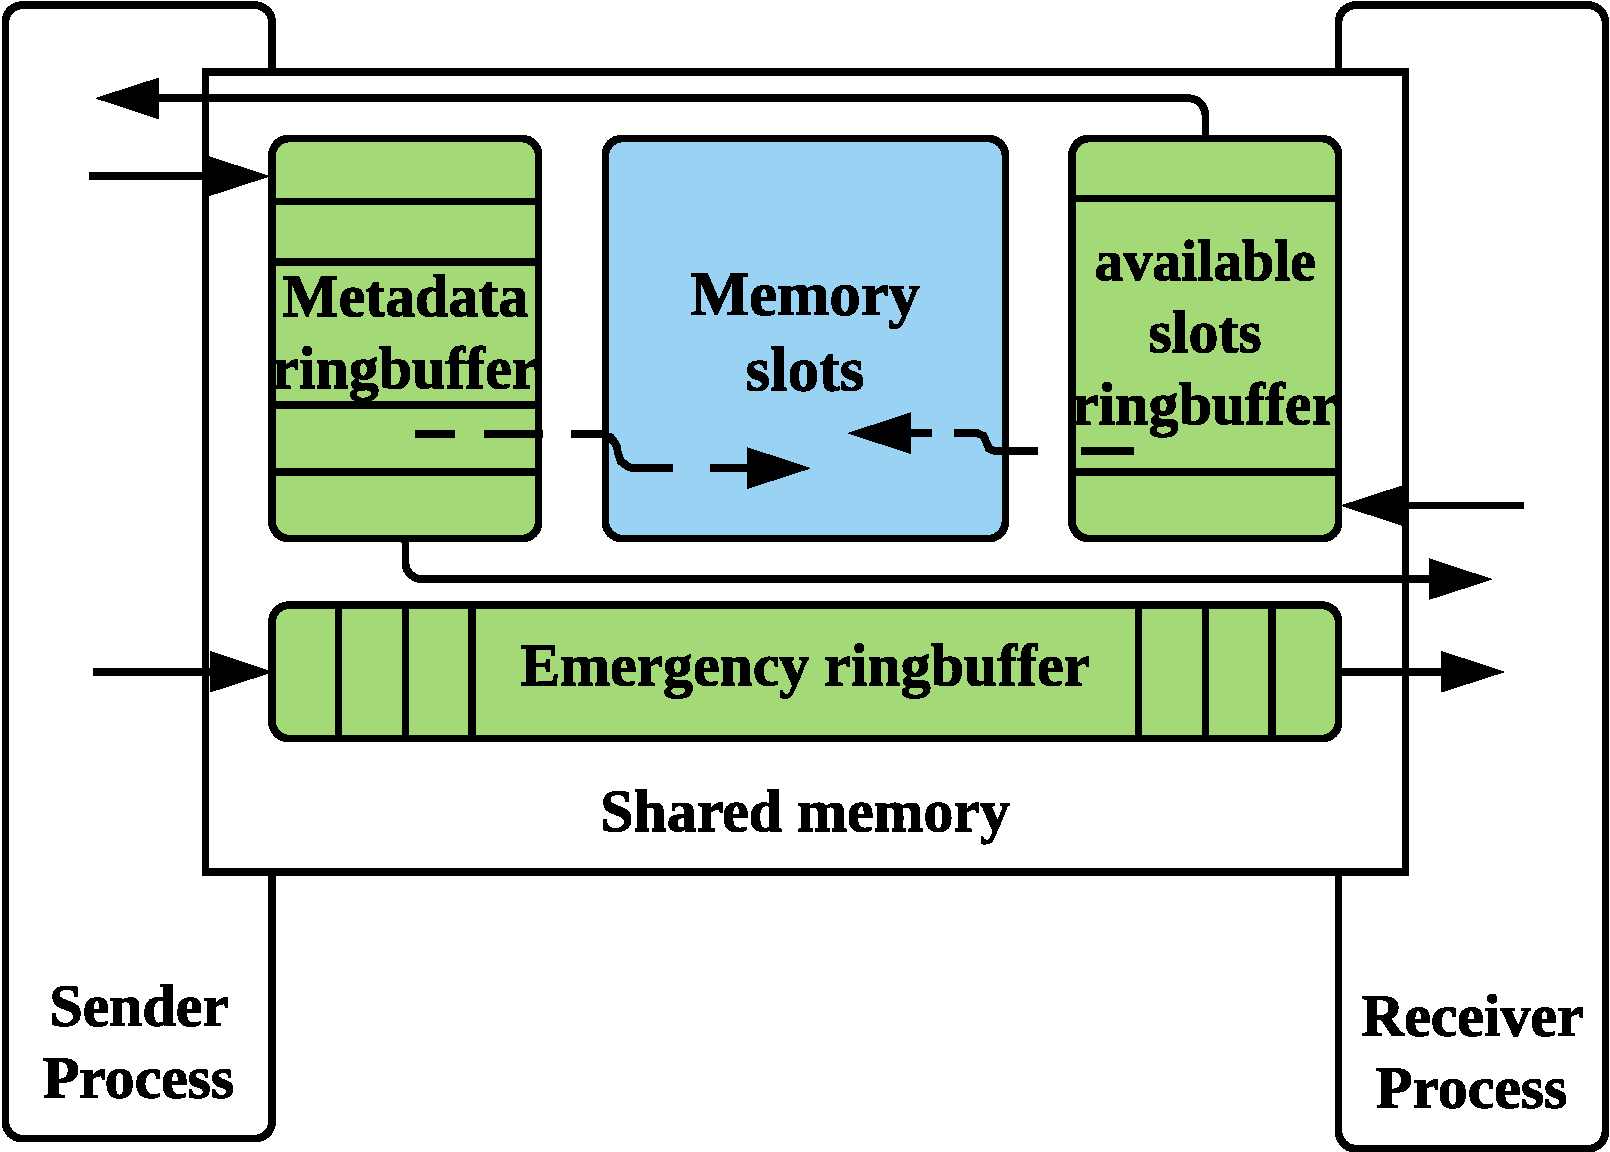
\includegraphics[width=0.4\textwidth]{images/locklessq}
	\caption{The structure of lockless queue (contain shared memory, 2 local ptr, isvalid flag and isdel flag).}
	\label{fig:locklessq-structure}
\end{figure}

In the previous section, we discuss requirements of the queue between a pair of communicating processes. A single sender enqueues data sequentially. At the same time, a single reader peeks and dequeues data at any position. In addition, the queue needs to support variable-sized data items to allow data copy from application send buffers when zero-copy is not applicable. In this section, we discuss a high performance lockless queue design.

As shown in Figure~\ref{fig:locklessq-structure}, a queue has three ring buffers and a data buffer pool in shared memory. Each ring buffer consists of equal-sized slots and enables unidirectional peer-to-peer communication. Two ring buffers are from sender to receiver, carrying socket \texttt{send} metadata and control messages respectively. Another ring buffer is from receiver to sender, holding available slots in the data buffer pool. If data of a \textit{send} operation is small enough to fit in a slot, it is piggybacked with metadata in the ring buffer. Otherwise, data buffers are allocated and chained to a linked list to hold data of arbitrary size. We use a pool of constant-size data buffers to simplify buffer allocation.

\parab{Credit-based ring buffer.}
Most ring buffer designs use atomic operations to maintain \textit{head} and \textit{tail} pointers that are shared between two endpoints. To eliminate atomic operations, we keep \textit{head} and \textit{tail} pointers locally in sender and receiver respectively.
To tell whether the ring buffer is full, the sender maintains a \textit{credits} count, indicating the number of unused items in ring buffer. When sender enqueues an item, it consumes a credit. When receiver dequeues an item, it increments a counter locally, and writes a \textit{credit return flag} in sender's memory once the counter exceeds half the size of ring buffer. The sender regains credits upon detecting the flag.

Metadata and data of the ring buffer resides in receiver's memory. Each slot in the ring buffer has a \textit{isvalid} flag. Sender sets \textit{isvalid} after writing the data. Receiver polls \textit{isvalid} to find a non-empty slot, then copies data from the slot, finally clears \textit{isvalid}.

\parab{Consistency between data and metadata.}
For intra-server communication, one may think that out-of-order execution may mandate the use of memory fence instructions. Actually, memory fence is unnecessary because modern processors provide a strong inter-core memory consistency. X86 processors from Intel and AMD provides total store ordering~\cite{sewell2010x86,intel-manual}, which implies that two writes are observed in the same order as they were written, and that reads are never postponed in out-of-order execution. Only a single cache migration is needed per send or receive operation. In the intra-server case, our synchronization-free ring buffer achieves $30~M$ messages per second throughput and $100~ns$ end-to-end latency, while a ring buffer based on memory fence can only sustain throughput around $10~M$ messages per second.
For inter-server communication, the only RDMA verb we use is one-sided posted \texttt{write}, so the ring buffer is wait-free on both sender and receiver.

\parab{Pick from middle of queue.}
In order to support picking data for a specific FD, receiver needs to traverse non-empty slots and dequeue a slot from any position in ring buffer. During traversal, receiver iterates slots from \textit{tail} until the first slot whose \textit{isvalid} is not set, which corresponds to the \textit{head}. Consequently, receiver cannot clear \textit{isvalid} when a non-tail slot is dequeued. We add an additional \textit{isdel} flag to each slot. When a slot is dequeued, its \textit{isdel} flag is set. If the slot at \textit{tail} has \textit{isdel} set, we clear both \textit{isvalid} and \textit{isdel}, increments \textit{tail} and repeats this step.


%As stated in section \ref{subsubsec:data_trans}, our lockless queue i.e. ring buffer is used for direct data transmission between two processes, and is used for message passing between process and the monitor. To recap, lockless queue in \libipc is used to support one-one connection in shared memory.

%The structure of lockless queue is shown in Figure~\ref{fig:locklessq-structure}. We leverage ring buffer as the data structure of the queue. Each slots of the queue is 16 bytes. Both sender and the receiver have a pointer stored locally. We denote the pointer of sender side as \textit{head}, and the receiver one as \textit{tail}. The sender pushes new items to the location pointed by head and increases the head while the receiver pops items according to its own tail and increases its tail.  In order to know whether the slot pointed by \textit{head} or \textit{tail} is available, we put a \textit{isvalid} flag in each of the slot. When sender pushes the item, the flag is set while when receiver pops the item, the flag is cleared.

%In order to support ``pick'' from the middle of the queue, we add an additional ``isdel'' flag to each slot. When ``pick'' happens, ``isdel'' is set and ``isvalid'' is not changed. When receiver tries to pop an item from ``tail'', it iterate the ring buffer from tail and check ``isdel'' flag. If it is set, ``isvalid'' is set to false and ``tail'' is increased.



%To support variable size of messages, we allocate a memory pool in shared memory and set the pointer in message queue to the element in memory pool. We divide memory pool to 1KB blocks. The IDs of the available blocks are organized in another queue and are pushed by receiver (Receiver pops the item and releases the memory) and are consumed by sender. If the size of message is larger 1KB, multiple blocks are used and chained as a linked list. By doing so, we could avoid memory fragmentation and reduce the memory management contention between sender and the receiver. 

%It is common that the operation of the shared memory is protected by the \textit{memory fence} instruction in order to avoid the reorder caused by out-of-order execution on modern X86 CPU, which has expensive cost since it locks the memory bus. We make the observation that only write may be delayed according to the manual of Intel \cite{sewell2010x86,intel-manual}. By carefully adjusting the order of the instructions and removing \textit{memory fence}, the throughput of lockless queue could achieve 30M per second. 

%\subsubsection{Using RDMA for Inter-Server Ring Buffer}
%\label{subsec:rdma-ring-buffer}

%To communicate with RDMA capable peers, \libipc{} translates socket operations to one-sided RDMA \texttt{write} verbs. We implement a ring buffer between each pair of communicating processes using RDMA verbs. The difference between intra-server and inter-server ring buffer is memory access latency. In our intra-server ring buffer design, sender checks \textit{isvalid} bit of each item in ring buffer to determine whether the queue is full, and receiver also checks \textit{isvalid} bit to determine whether the queue is empty. In RDMA setting, either sender or receiver needs to use RDMA to check \textit{isvalid} bit remotely, incurring one round-trip delay per enqueue or dequeue.

%To avoid such delay, we design a \textit{credit-based ring buffer} for inter-server socket. Data of the ring buffer resides in receiver's main memory. Sender holds a tail pointer locally and receiver holds a head pointer locally. Sender maintains a number of \textit{credits}, indicating the number of unused items in ring buffer. When sender enqueues an item via RDMA \texttt{write}, it consumes a credit. When receiver dequeues an item, it increments a counter locally, and RDMA \texttt{write} a flag in sender's memory once the counter exceeds half the size of ring buffer. The sender regains credits upon detecting the flag. In this way, returning credits in batches amortizes RDMA messaging overhead for checking queue full. The only RDMA verb we use is one-sided posted \texttt{write}, so the ring buffer is wait-free on both sender and receiver. We did not use this design for intra-server because it doubles ring buffer size for a given queue capacity and affects memory locality.


\subsection{Scaling Shared Socket}
\label{subsec:fork}
Process fork and thread creation are ubiquitous in modern applications. 
Fork and thread makes sockets to be shared, and thus become a multiple producers or multiple consumers model. With a traditional mutual exclusion solution, the multi-process scalability of socket is limited. Our aim is to maximize the common-case performance while keeping compatibility with Linux socket semantics.

We make two observations: 1) Fork and thread creation are not frequent in high performance applications compared to connection setup and data transmission. 
and 2) It is uncommon that several processes \texttt{recv} concurrently from a shared socket, because the streaming semantics of socket makes it hard to avoid receiving incomplete messages. 
%For such producer-consumer scenarios, message brokers~\cite{hintjens2013zeromq,rabbitmq2017rabbitmq,kreps2011kafka} are typically used.

Based on the observation, we propose the following requirements to maximize the common-case performance of a shared socket:

\begin{enumerate}[noitemsep,nolistsep]
 \item \textbf{Synchronization-free.} With multiple potential senders and receivers, if only one pair of sender and receiver is active, the throughput and latency should be comparable with that of a sender-receiver pair.
 \item \textbf{Multi-sender scalability.} Multiple processes may send data concurrently through a shared socket. With multiple active senders and a single receiver, if the receiver is not a bottleneck, the throughput should scale.
 \item \textbf{Self-stabilization.} Certain operations (\textit{e.g.} \texttt{fork}) may slow down the system temporarily, but after that the throughput should converge back to normal.
\end{enumerate}

For compatibility with Linux semantics, we also need to ensure message ordering and liveness:
\begin{enumerate}[noitemsep,nolistsep]
\item \textbf{Single receiver ordering.} For a specific pair of sender and receiver, the received messages have the same ordering as they were sent.
\item \textbf{Multiple receiver ordering.} The order of \texttt{send} and \texttt{recv} operations for one sender and multiple receivers should be linearizable. If receiver $R_1$ already receives $D_1$, then receiver $R_2$ calls \texttt{recv} and gets $D_2$, we guarantee that $D_1$ is sent before $D_2$.
\item \textbf{Deadlock-free.} If a socket buffer is not empty when \texttt{recv} is called by one or more receivers, at least one receiver should get data.
\item \textbf{Starvation-free.} If a sender keeps sending, any receiver trying to \texttt{recv} will eventually get data.
\end{enumerate}

Our scalable socket design can be divided into four parts: a) \texttt{send} and \texttt{recv}, b) adding new senders and receivers (\texttt{fork} and \texttt{pthread\_create}), c) connection creation and d) connection close.

\subsubsection{Send/Recv Operation}
\label{subsubsec:fork_rdwr}

\begin{figure}[t]
	\centering
	
\includegraphics[width=0.3\textwidth]{images/fixme}
	\caption{A socket connection is shared by three processes. $S$ is the sender, $R_1$ is the previous designated receiver and $R_2$ is the new receiver that takes over the socket.}
	\label{fig:fork-takeover}
\end{figure}

In this section, we assume that a socket is already connected and the number of senders and receivers are constant. We discuss adding senders or receivers in the next section.

\parab{Multiple concurrent senders.}
In order to avoid synchronization, we create queues between \emph{every} pair of senders and receivers. %The queues form a bipartite graph between senders and receivers. 
Each receiver polls messages from all sender queues in a round-robin manner. Therefore, the multi-sender throughput can scale.
%Figure \ref{fig:fork-bipartitegraph} shows a sample of the shared-memory buffers between senders and receivers for one connection.

\parab{One exclusive receiver.}
Each sender, though has a queues to every receiver, designates only a single receiver with exclusive access to the socket and only send data through the corresponding queue. 
In the common cases with only a single active receiver, the performance would be the same as one-to-one communication. 
%It is challenging for the sender to choose a receiver, since the chosen one may not call \texttt{recv}, while other receivers may be under starvation. 

\parab{How to take over.}
When a non-designated receiver attempts to \texttt{recv} from the socket, it sends a \textit{takeover request} to the sender. 
Up receiving the request, the sender %processes takeover requests in FIFO order to avoid starvation and 
designate the requester as the new exclusive receiver and remove the status from the old designated receiver. 
%Another challenge is that when a receiver should send a takeover request. 
%Each receiver maintains a flag locally to indicate whether it is designated by the sender. The flag is flipped when the receiver gets takeover request or completion from sender. When a receiver tries to \texttt{recv} and finds itself not designated, it sends a takeover request to sender. Before the receiver becomes designated, the takeover request is sent only once.

\parab{Remaining data in queue.}
A challenge arise when there is remaining data in the queue when a receiver requests to take over the socket. %We need to ensure that all the remaining data can be received by the new receiver. 
%Because multiple sockets share a queue from sender to each receiver, and different sockets have different designated receivers, the new receiver cannot access the queue from the old receiver directly. Instead, 
The remaining data needs to migrate from the old active queue to the new active queue. When the sender processes a takeover request, it first forwards it to the current receiver. Upon receiving takeover request, the current receiver returns all remaining data to sender via \textit{takeover completion} messages, which the sender forwards to the new receiver. During migration, the sender blocks \texttt{send} operations and takeover requests to ensure message ordering. The takeover procedure is shown in Figure~\ref{fig:fork-takeover}.


%\begin{figure}[t]
%	\centering
%	
\includegraphics[width=0.3\textwidth]{images/fixme}
%	\caption{This figure shows a stable connection handled by multiple senders and receivers.}
%	\label{fig:fork-bipartitegraph}
%\end{figure}

\subsubsection{Fork and Thread Creation}
\label{subsubsec:fork_fork}


\begin{figure}[t]
	\centering
	
\includegraphics[width=0.3\textwidth]{images/fixme}
	\caption{Message flow during \texttt{fork}.}
	\label{fig:fork-fork}
\end{figure}


The first challenge with fork and thread creation is how to identify and isolate parent and child processes. As shown in Figure~\ref{fig:fork-fork}, when the application calls \texttt{fork}, \texttt{clone} or \texttt{pthread\_create}, \libipc{} first generates a secret for pairing, then invokes the corresponding system call. After fork, parent and child independently creates a \textit{bootstrap socket} to the monitor and sends the secret (child inherits parent memory space and knows the secret). The monitor can thus pairs the child process with the parent. 
To maintain isolation between parent and child, monitor creates new shared memory queues to replace all queues in \emph{both} parent and child. We do not reuse queues due to potential isolation violation. %The monitor then sends credentials of new queues to parent and child via bootstrap sockets. 
Each peer process is also notified of the new queues and the new process. From then on, parent and child processes have isolated queues to the monitor and peers.

%A harder challenge comes from socket connection sharing between parent and child processes. 
Upon fork, each connection needs to add a sender to the sending direction and a receiver to the receiving direction. A major challenge is how to handle the remaining data in the original send and receive queues.

%For each unidirectional queue, we discuss the behavior of related processes in four cases:
%\begin{enumerate}
%	\item A sender process itself forks.
%	\item A receiver of a sender process forks.
%	\item A receiver process itself forks.
%	\item A sender of a receiver process forks.
%\end{enumerate}

%The general process of fork is that after monitor is notified of the fork, it creates shared memory between the newly created process and all the processes which previously have connections with the parent process. The key challenge lies in the fork is that how to deal with the existing data in the connection to guarantee the order requirements.

\parab{Receiver fork.}
First we look at the simpler case when a receiver forks. Recall that only one receiver has exclusive access to a socket, as stated in Sec.~\ref{subsubsec:fork_rdwr}. The parent process inherits receive permission and the child process is initially not the exclusive receiver after fork. When a sender receives fork notification of its peer, it copies all data from original queues to new queues of the parent process.

\parab{Sender fork.}
Next we look at the more complicated case when a sender forks. We need to guarantee that all the data sent prior to \texttt{fork} is consumed before the data sent after \texttt{fork}. 

It is inefficient to block the senders until remaining data in the queue is consumed. Our solution is to drain the original queue first before switch to the new queues. At fork time, we detach the original sender's shared memory queue and create two new queues, one for the parent and one for the child. Both parent and child can send data to new queue as usual. When the receiver is notified of the fork, it keeps track of the original queue and consumes all data in it before activating new queues. Note that the parent or child may fork again before the original queue is drained. With this in mind, the receiver maintains a forest data structure to track dependency of queues. The root of each tree in the forest is the oldest queue to receive from. Each non-leaf node has two children indicating the new queue of parent and child processes. If a non-leaf root queue becomes empty, it will be removed, and the two children queues will be promoted to roots.

\parab{Takeover During Fork.}
There is a subtle issue remaining. After a sender forks, the receivers still need the takeover mechanism to arbitrate remaining messages in the original shared memory queue. However, both parent and child senders have dropped the original queue and will not respond to takeover requests. A similar situation occurs when a sender process dies. Our solution is to let the receivers use atomic operations to compete for remaining data in the original queue. Since this case rarely happens, the performance of the overall design is not affected.


%Things become much more complicated when cases 1,4 happens after cases 2,3 happening. After receiver forks, the unique sender is responsible for receiving ``takeover message'' and resend the data to new receivers. However, if sender forks following the receiver forks, according to the methods we mentioned above, there is no sender responsible for processing ``takeover message''. Our solution is that we require the receivers to poll the data from the old shared memory queue and compete for data. Since this case rarely happens, the performance of the overall design is not affected.

\subsubsection{Connection Creation}
\label{subsubsec:fork_new}

%A connection created after \texttt{fork} cannot be accessed by its sibling process, while 
A connection created by a thread can be accessed by all threads in the same process. To minimize state sharing, \libipc assigns a unique file descriptor (FD) space to each thread, so that each thread can allocate FDs locally. 
% and determine which thread a FD belongs to. 
During connection creation, \libipc does not share the FD eagerly with other threads, because most threads in existing applications do not use connections created by other threads.
When a thread do want to accesses a FD that belongs to another thread, \libipc sends a message to the owner thread and requests sharing the FD. This procedure is exactly the same as sharing existing connections during thread creation (Sec.~\ref{subsubsec:fork_fork}). %The sharing procedure only happens once for every connection and thread. Sharing existing connections eagerly during thread creation is an optimization. First, children threads are more likely to use existing connections than siblings. Second, batch processing improves performance.

\subsubsection{Connection Close}
\label{subsubsec:fork_close}

%Close is the operation that all of the processes leave the connection. The synchronization is  especially challenging since all the processes are run in parallel. One challenge lies in file descriptors are managed by decentralized processes and are possibly reused. One process close a connection while the others are doing compute intensive tasks is a case. It is possible that the file descriptor of the old process is reused and a new connection is setup with the same file descriptor. The other process may notice the close of the old connection and also call close on its own side, which lead to the new connection setup by the previous process closed due to the match of same file descriptor. 

%To satisfy the synchronization requirements, the close function call is all completed by message passing. The caller of close need to wait for ACK from all the other peers before release resources. i.e. the status of the connection.

%\parab{Broadcast.}
When a process calls \texttt{close} or \texttt{shutdown}, all its peers cannot send to or receive from the process. In this sense, closing a shared socket is a multicast operation to notify the peers. A challenge arise when \texttt{close} is interleaved with \texttt{fork}. Since \texttt{fork} and \texttt{close} do not commute~\cite{clements2015scalable}, we need a rule to determine their partial order. We make the choice that the ordering is determined by the initiator of \texttt{close}. If a process calls \texttt{close} before receiving fork notification, it will piggyback close notification with fork completion to both parent and child processes.

%\parab{Handshake before releasing resource.}
%Another challenge is caused by FD reuse after close. As stated in Sec.~\ref{subsec:socket-api}, a FD is deleted after receiving shutdown message of both directions. With multiple processes sharing a connection, after one process calls \texttt{close}, others can still use the connection. Consequently, a process deletes a FD only after receiving shutdown messages of both directions from all peers of the FD.

%Another challenge lies in the close of a connection is that close is a broadcast operation while send/receive is sent to a specific process. Besides, fork and close are immutable operations while the scalability requirements of the system impose the constraint that all the operations run asynchronously. As a result, a rule to determine the partial order is required.

%In \libipc, we make the choice that the order of fork and close is determined at the start point of the fork operation and the end point (after receiving all the ACKs). By making this choice, when a process waiting fork close ACK encounters fork message, it could send a separate close request to newly created process, which guarantees all the processes closed.


\subsection{Cooperative Multitasking}
\label{subsec:process-mux}

\parab{Event notification.}
To minimize context switch, \sys{} runs in user mode and uses cooperative multitasking to multiplex processes on CPU cores. Coordination and delegation based on message passing also requires processes to respond to messages promptly. However, processes may execute application code without calling \libipc{} for a long time. To tackle this issue, we design a \textit{signal} mechanism analogous to interrupts in operating systems. Event initiators  first poll the receive queue for a period of time for ack. If no reply, it sends a Linux \texttt{signal} to the receptor and wake up the process.

The signal handler, registered by \libipc{}, first determines whether the process is executing application or \libipc{} code. To determine this, \libipc{} sets and clears a flag at entry and exit of the library. If signal handler finds that the process is in \libipc, it does nothing and \libipc{} will process the event before returning control to the application. Otherwise, the signal handler immediately processes messages from the emergency queue to the monitor, then return control to the application. 
%Because \libipc{} is designed to be fast and non-blocking, message passing initiators will soon receive the response.

\parab{Polling and sleep.}
When an application calls non-blocking socket operations, \libipc{} polls queues of the specified FD and the emergency queue to the monitor, then returns immediately. For blocking operations (\textit{e.g.} blocking \texttt{recv}, \texttt{connect} and \texttt{epoll\_wait}), \libipc{} first polls the queues once. If the operation is not completed, \libipc{} calls \texttt{sched\_yield} to yield the processor to other processes on the same core. %As stated in Sec.~\ref{subsec:bottleneck}, context switch in cooperative multitasking only takes 0.4~$\mu$s. However, an application may wait a long time for an external event, making frequent wake-ups wasteful. In this regard, we count consecutive wake-ups which does not process any message, and puts the process to sleep when this reaches a threshold. 
As mentioned in \ref{subsec:data_trans}, if \libipc{} continues to yield for several rounds, it will put itself into sleep. Before sleeping, it sends a message to the monitor and all peers, so they can wake up the sleeping process after sending a message via shared-memory queue.

%\parab{Exit.}
%When a process exits, the \texttt{atexit} handler of \libipc{} notifies the monitor and all peers to close connections and mark the queues as dead. However, a process may crash or get killed. In this case, monitor detects process death via \texttt{SIGHUP} of the bootstrap socket (Sec.~\ref{subsubsec:fork_fork}) and notify its peers. When a process switches to \texttt{daemon} mode or \texttt{execve} another program, it first follows the process exit procedure, then calls the system call. After that, \libipc{} is re-initialized.


\subsection{Zero Copy}
\label{subsec:zerocopy}

\begin{figure}[t]
	\centering
	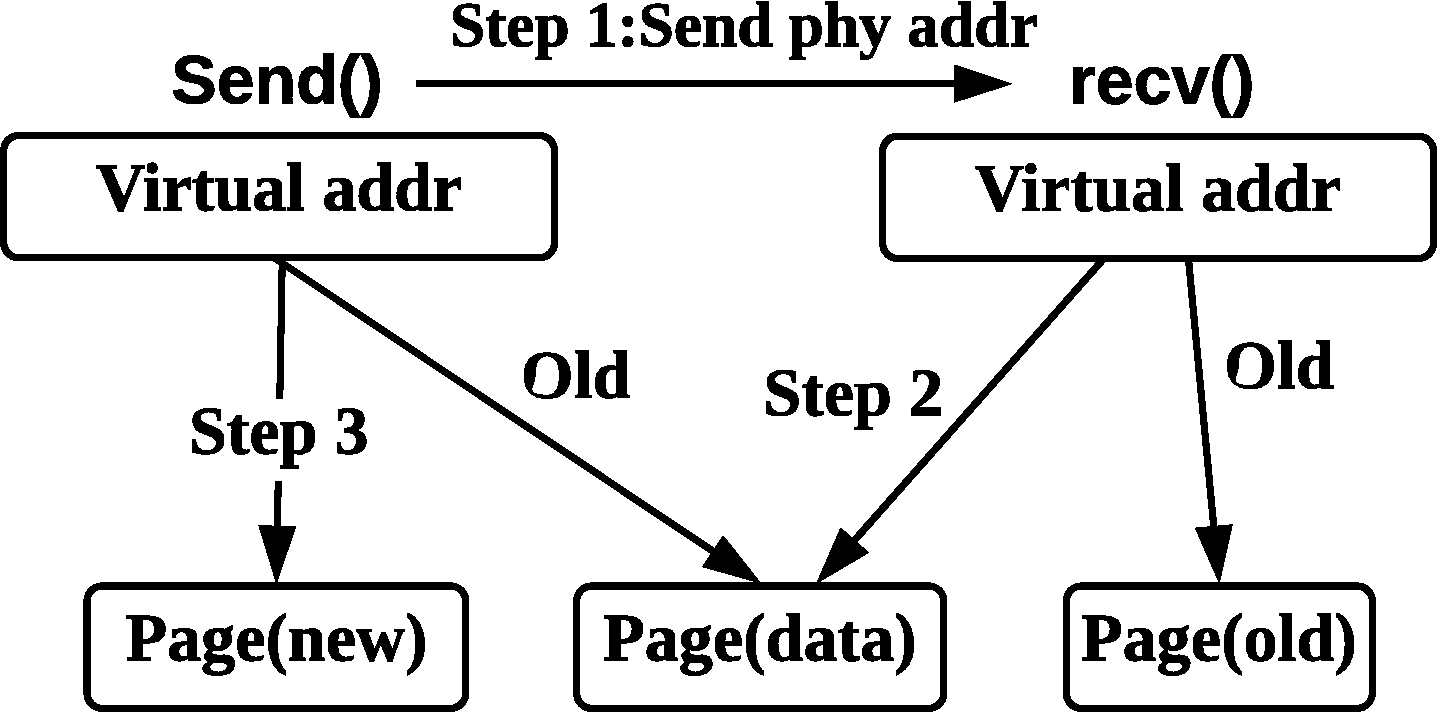
\includegraphics[width=0.3\textwidth]{images/zerocopy}
	\caption{Zero-copy theory of operation.}
	\label{fig:zerocopy}
\end{figure}

The main challenge for zero copy is to maintain the semantics of socket API, as discussed in \ref{subsec:challenges}.
%A sender may write the send buffer after non-blocking \texttt{send}, and the receiver does not know the receive buffer before \texttt{recv}.
Fortunately, virtual memory provides a layer of indirection, so we can remap virtual address of a buffer to another physical page if the data occupies entire 4~KiB pages.
We wrap around \texttt{malloc} and \texttt{realloc} functions and allocate 4~KiB aligned addresses for large allocations, so most buffers will align to page boundary.
If the size of send message is not a multiple of 4~KiB, the last chunk of data is copied on \texttt{send} and \texttt{recv}.

\subsubsection{Zero Copy for Intra-Server Socket}
\label{subsec:zero-copy-intra}

\parab{Page remapping.}
As shown in Figure~\ref{fig:zerocopy}, for \texttt{send} operation, \libipc{} invokes the kernel to get an encrypted physical address of send buffer and send the address to receiver via user-mode shared-memory queue.
The address is encrypted to prevent unsolicited mapping of arbitrary pages.
Because the sender may read the buffer after \texttt{send} or send the buffer to multiple receivers, the physical page cannot be remapped.
Additionally, \texttt{send} needs to write-protect the buffer because the receiver needs to read it.
On the receiving side, \libipc{} invokes the kernel to remap the encrypted physical address to the application-provided receive buffer.
\texttt{recv} also needs to write-protect the buffer because it is shared by the sender and potentially multiple receivers.

\parab{Minimize copy-on-write.}
A challenge arises when sender writes the buffer after \texttt{send}.
Existing zero-copy socket designs~\cite{thadani1995efficient,chu1996zero} use copy-on-write. %Copy is required because the sender may read the non-written part of the page.
Because most applications reuse the buffer for subsequent send operations, copy-on-write is invoked in most cases, making zero-copy essentially useless on sender.
Our observation is that most applications overwrite entire pages of the send buffer via \texttt{recv} or \texttt{memcpy}. %so it is unnecessary to copy old data when the first byte of the page is written.
Zero-copy by \texttt{recv} already remaps the buffer without triggering copy-on-write.
We add preamble code to \texttt{memcpy} in both \libipc{} runtime and compiler inline library. 
For page-aligned copy to \libipc{} buffers, the preamble code invokes the kernel to remap new pages and disable write protection.

\parab{Page pool in user space.}
A second challenge is that page remapping requires the kernel to allocate and free pages for each \texttt{send} and \texttt{recv}. Page allocation in kernel acquires a global lock, therefore it is inefficient. Instead, \libipc{} manages a pool of free pages in each user-mode process.
We add to the kernel a system call to convert virtual addresses in the pool and encrypted physical addresses.
\libipc{} also tracks the origin of received zero-copy buffers.
After finish accessing the remapped page, if the page is from another process, \libipc{} sends a message to the original process to return the buffer.

\subsubsection{Zero Copy RDMA}
\label{subsec:zero-copy-rdma}

We use physical addresses in RDMA verbs to eliminate memory registration and address translation overhead, as recommended by NIC documentation~\cite{mellanox}. During connection initialization, the receiver prepares a huge-page buffer for receiving zero-copy messages. The sender manages free pages in the receive buffer. For \texttt{send}, \libipc calls the kernel to get physical address of send data buffer. it also allocates pages from receive buffer as remote address for RDMA \texttt{write}, and attach the address in metadata message in ring buffer. Upon \texttt{recv}, \libipc calls the kernel to map physical pages in metadata message to \texttt{recv} buffer address. 
%For security, kernel validates that page numbers are in the huge-page receive buffer. 
Same as intra-server zero-copy communication, when the receiver stops using the buffer, it is returned to the sender.

\subsubsection{Zero Copy TCP}
\label{subsec:zero-copy-tcp}

To remove data copy between \libipc{} and NIC, the payloads of sent and received packets need to align at 4~KiB page boundary. We leverage scatter-gather support in modern NICs~\cite{mellanox} to separate packet header from application payload.
%During initialization, \libipc{} queries IP and Ethernet MAC address from the kernel and constructs a packet header template.
For \texttt{send}, \libipc{} constructs a packet header to a NIC send work request, then fills in the payload buffer address from application. 
For receiving data, in background, \libipc{} issues NIC receive work requests with a 54-byte buffer to hold exactly Ethernet, IPv4 and TCP headers, followed by a page-aligned buffer to hold payload.
%In corner cases where the received header length is not 54 bytes, \libipc{} reassembles the packet.
Upon \texttt{recv}, the payload buffer is remapped to application.


%\subsection{Inter-Server Socket}
%\label{sec:inter-server}

%Previous section discussed inter-process socket in a same server. For inter-server socket, \libipc{} determines whether or not the peer supports RDMA. If so, \libipc{} translate socket operations to one-sided RDMA \texttt{write} verbs. Otherwise, \libipc{} calls a light-weight user-mode TCP/IP stack to communicate with standard TCP/IP endpoints. In both cases, we achieve zero copy and scalability with number of threads and number of connections.


\subsection{Light-weight TCP/IP in User Space}
\label{subsec:lwip}

%\sys{} needs to communicate with standard TCP/IP endpoints without RDMA support. We leverage Receive-Side Scaling (RSS) in modern NICs to distribute incoming and outgoing connections to the NIC queues of listening processes. For outgoing connections, \libipc{} chooses a source port such that received packets will be distributed to its own queue. For incoming connections, the monitor process configures NIC indirection table~\cite{mellanox} when a process binds an external IP address. Similar to intra-server, when load imbalance occurs, idle listeners steal new connections via monitor. Because the NIC still distributes packets to the original listener, it forwards received packets via shared memory queue.

%\sys{} needs to communicate with standard TCP/IP endpoints without RDMA support. There has been extensive work on user-space socket and TCP/IP stack in both academia~\cite{dunkels2001design,rizzo2012netmap,huang2017high} and industry~\cite{libvma,openonload,dbl}. However, most of these works do not optimize for a large number of concurrent connections, require locks for multi-thread applications, and do not support zero copy without application modification.

%A network stack is logically composed of three layers: the socket API for applications, TCP/IP protocol for reliable transmission and packet send/receive interface with NIC hardware. Our intra-server socket design in Sec.~\ref{sec:intra-server} applies directly to inter-server socket API. 

%With a large number of concurrent connections, per-connection states in TCP/IP protocol stacks not only consumes host memory, but also reduces memory access locality. To save memory, light-weight TCP/IP stacks~\cite{dunkels2001design} do not pre-allocate send and receive buffers of TCP window size. But each connection still needs send and receive bitmaps to track out-of-order and lost packets, and selectively retransmit them. We modify LwIP~\cite{dunkels2001design} to incorporate MELO~\cite{lu2017memory}, a memory-efficient loss recovery mechanism that share bitmaps among connections. In this way, bitmap memory footprint is amortized to $\approx20$ bytes per connection.

%For multi-thread applications, \libipc{} uses thread-local storage for states and file descriptors to eliminate locks. Each thread owns exclusive work request and completion queues to communicate with the NIC. In order to avoid TCP state sharing among threads, \libipc{} designates one thread with exclusive access to each TCP socket. If other threads access the file descriptor, it sends a takeover message to the owner thread, as in Sec.~\ref{subsubsec:fork_rdwr}.

%To improve multi-process scalability of TCP servers, we leverage Receive-Side Scaling (RSS) in modern NICs to distribute incoming and outgoing connections to the NIC queues of listening processes. For outgoing connections, \libipc{} chooses a source port such that received packets will be distributed to its own queue. For incoming processes, the monitor process configures NIC indirection table~\cite{mellanox} when a process binds a non-local IP address. Each process maintains TCP connections locally. However, listeners may need to migrate new connections under load imbalance. To this end, each listener maintains a \textit{backlog} of received new connections which has not been \texttt{accept}ed by the application. When the backlog overflows, it forwards the new connection to the monitor. When an idle process calls \texttt{accept} while backlog is empty, it requests from the monitor. Then, the overloaded process will forward received packets of the migrated connection to the idle process via shared-memory queue.
